% !TEX root = deplump.tex
\section{Experiments}
\label{sec:experiments}

As the performance of batch deplump was established relative to other lossless compressors for a variety of datatypes in \citep{Gasthaus2010}, we focus our experiments on establishing a) that the approximations to inference in the sequence memoizer combined in this paper in order to make deplump a streaming compressor do not significantly adversely affect compression performance, b) that the resulting compressor can indeed compress extremely long sequences as the asymptotic guarantees would suggest it should, and c) what settings of the approximation parameters produce the best compression performance.

All of the experiments included in this paper use a complete Wikipedia text content dump \citep{Wikipedia} as a test corpus (26.8Gb uncompressed, 7.8Gb gziped and ??Gb paq9a'ed, each with default parameters, and 3.9Gb deplumped).  To establish what approximation parameters produce the best compression results we first ran streaming deplump on the first 100Mb section of the corpus limiting the depth to two different values ($D=16$ and $D=1024$) with a fixed limit on the number of nodes in the tree ($L=10^6$).  We observed that in both cases only very few nodes had high total counts ($c > 8,192$) suggesting that it might be possible to set the count upper bound to a relatively low value ($k= 8,192$) without significant compression performance degradation.  That compression performance should not be affected by a reasonable count bound follows intuitively from the fact that in byte sequences $|\Sigma| = 256$ and setting $k=10,000$ is similar in effect to using 10,000 observations to estimate a 256 element discrete distribution.  To ensure that compression performance did in fact not suffer, we compressed ten 100Mb subsections of the corpus (sampled randomly with replacement) for multiple values of $k$ between 128 and 32,768 (fixing $L=10^6$ and $D=16$).  We observed that average compression performance varied insignificantly over different values of $k>?$ .

 In each of the following experiments, subsections of the corpus were sampled with replacement.  In the first experiment the sampled subsections were all of size 100Mb, while in the second the sampled subsections varied in length.  In the first experiment, the interplay between limiting the number of nodes in the tree and restricting the depth of the tree was explored (results for which are shown in Figure~\ref{fig:varying_depths}).  Here $k$ was set to 8,192, while $L$ and the depth of the tree $D$ were varied as indicated in the figure.  In the second experiment, the interplay between stream length and node limit was explored (Figure~\ref{fig:varying_stream_length}).  In this experiment $k$ remained fixed at the same value and the depth was set to $D=16$ while $L$ varied as shown in the figure.  

Figure~\ref{fig:varying_depths} indicates that compression performance becomes essentially indistinguishable for depth restrictions greater than $D=10$.  However, this figure also suggests that compression performance almost always improves as a function of the number of nodes in the tree for depths 6 and greater.  Figure~\ref{fig:varying_stream_length} illustrates that the algorithm not only scales to very long sequences, but average compression performance continues to improve as the sequence grows.  Using a large value of $L$ appears to be beneficial for very long sequences.

\begin{figure*}[t] 
	\begin{center}
		\scalebox{.6}{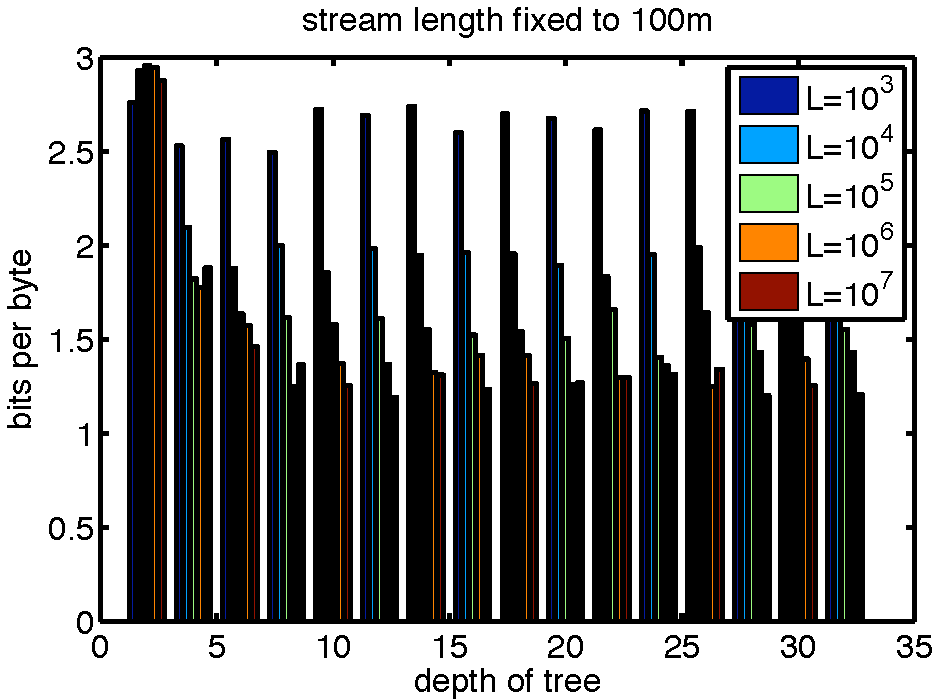
\includegraphics{figs/varying_depths.pdf}} % [clip=true, viewport= 1in 1in 9in 9in]
		\caption{Performance averaged over 10 random sections  100Mb sections of the corpus for varying fixed depths and number of allowable nodes ($L$) }
		\label{fig:varying_depths}
	\end{center} 
\end{figure*} 

%\begin{figure*}[t] 
%	\begin{center}
%		\scalebox{.6}{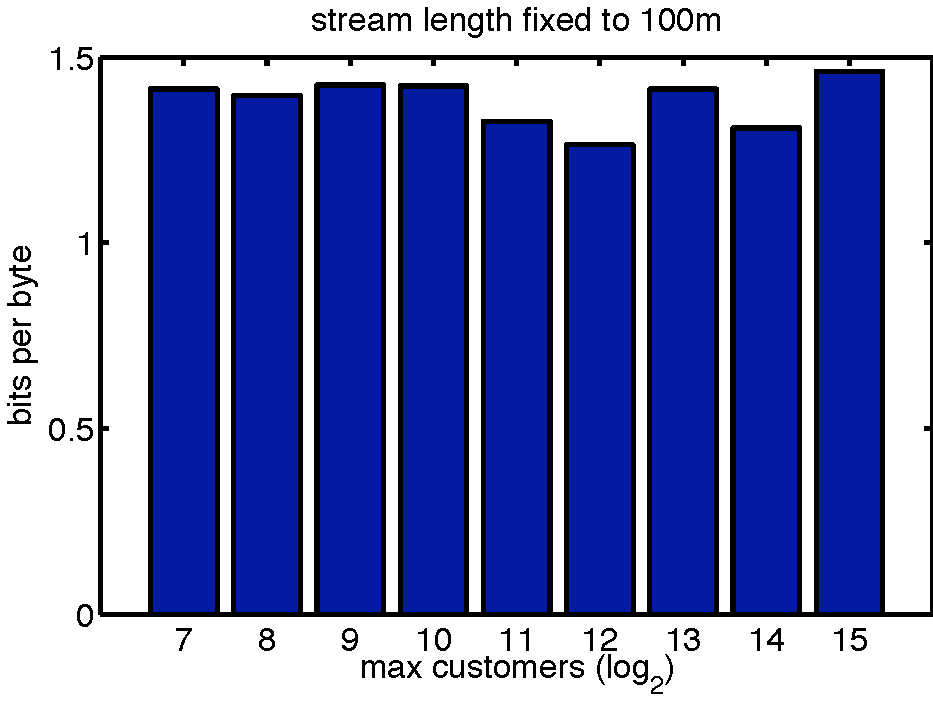
\includegraphics{figs/varying_max_customers.pdf}} % [clip=true, viewport= 1in 1in 9in 9in]
%		\caption{Performance for varying max allowable customers $k$.}
%		\label{fig: varying_max_customers}
%	\end{center} 
%\end{figure*} 

\begin{figure*}[t] 
	\begin{center}
		\scalebox{.6}{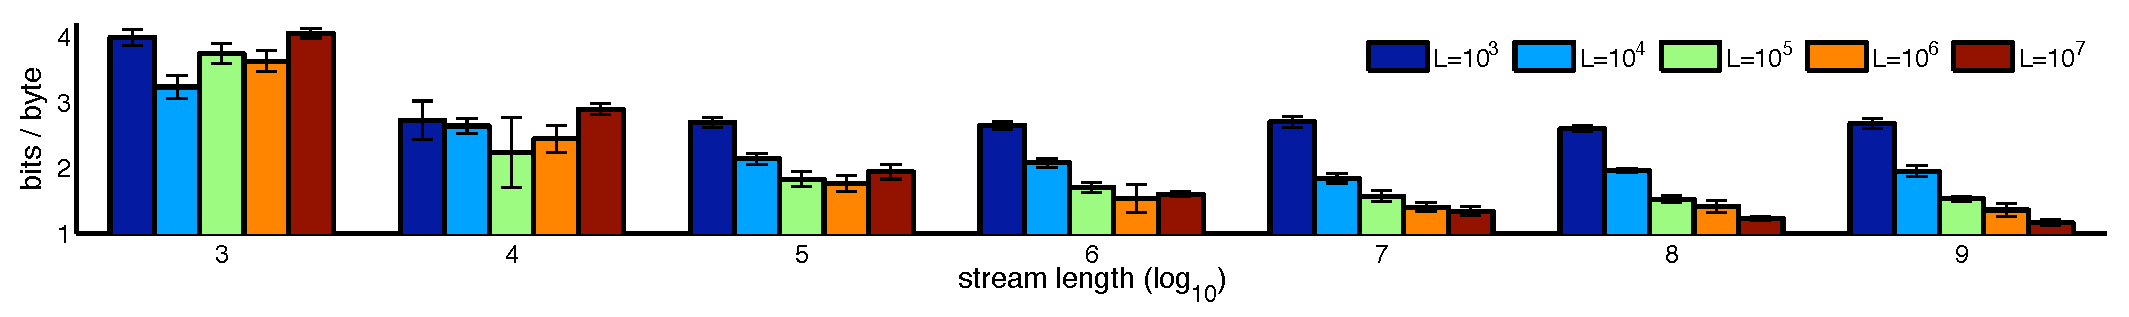
\includegraphics{figs/varying_stream_length.pdf}} % [clip=true, viewport= 1in 1in 9in 9in]
		\caption{Performance for varying stream lengths and number of allowable nodes ($L$).}
		\label{fig:varying_stream_length}
	\end{center} 
\end{figure*} 


%\begin{figure*}[t] 
%	\begin{center}
%		\scalebox{1}{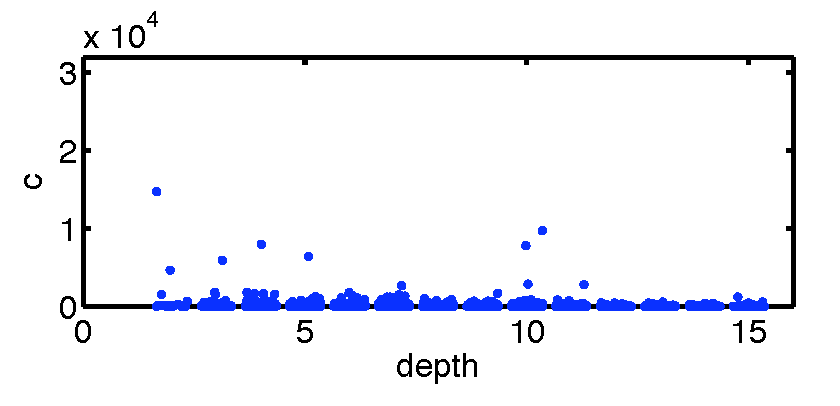
\includegraphics{figs/scatter_16.pdf}} % [clip=true, viewport= 1in 1in 9in 9in]
%		\caption{Scatter plots to explore the relationship between the depth of a node and the total count}
%		\label{fig:restaurant_plots}
%	\end{center} 
%\end{figure*} 

%\begin{figure*}[t] 
%	\begin{center}
%		\scalebox{1}{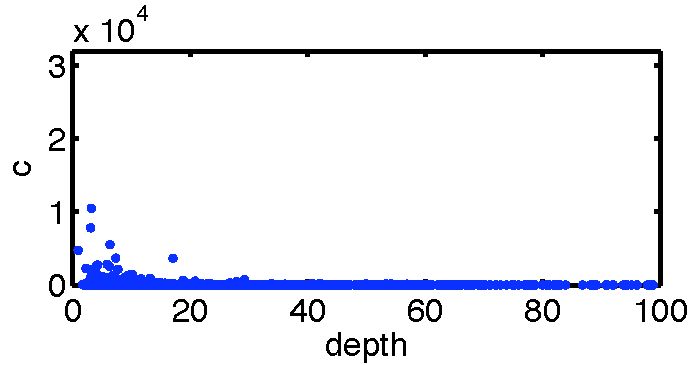
\includegraphics{figs/scatter_1024.pdf}} % [clip=true, viewport= 1in 1in 9in 9in]
%		\caption{Scatter plots to explore the relationship between the depth of a node and the total count}
%		\label{fig:restaurant_plots}
%	\end{center} 
%\end{figure*} 
